\chapter{\label{chap:previo}Infraestrutura de \textit{Fuzzing} e Estudo das Fontes de Realimentação}

Este capítulo descreve o trabalho já realizado. Antes de construir o gerador de programas definitivo, foi necessário decidir qual sinal do processador orientará a exploração, pois essa escolha determina o que o \textit{fuzzer} considera um comportamento novo. A \cref{sec:previo-fontes} apresenta os sinais levantados como candidatos. A \cref{sec:previo-impl} descreve a infraestrutura de \textit{fuzzing} construída sobre o RISCOF para compará-los. A \cref{sec:previo-exp} apresenta os experimentos e seus resultados, e a \cref{sec:previo-remarks} reúne as considerações que orientam a continuidade do trabalho.

\section{Sinais candidatos a realimentação}\label{sec:previo-fontes}

Um \textit{fuzzer} orientado por cobertura depende de um sinal que indique se um programa exercitou algo ainda não observado (\cref{sec:bg-fuzzing}). O Encarsia \citep{encarsia} mostrou que essa escolha não pode ser presumida: as métricas de dois \textit{fuzzers} conhecidos não alteraram o conjunto de falhas que eles encontraram. Por isso, cinco alternativas foram levantadas e instrumentadas, de modo que todas sejam registradas em cada execução e possam ser comparadas sobre os mesmos programas.

\begin{description}
    \item[Sem realimentação.] Cada programa é gerado do zero, e nenhuma informação da execução influencia o seguinte. Essa alternativa é a linha de base: como \textit{fuzzers} sem realimentação encontraram as mesmas falhas que suas versões guiadas \citep{encarsia}, um sinal só se justifica se superar a geração aleatória.

    \item[Cobertura de código do SystemVerilog.] O Verilator registra quais linhas e ramos do RTL foram avaliados. É o sinal disponível sem esforço adicional na infraestrutura do RS5 e representa as métricas estruturais: mede o que está escrito no código, e não as situações em que o processador se encontrou.

    \item[Estado do \textit{pipeline}.] A cada ciclo, uma sonda comprime em 40 bits os sinais de controle que descrevem os mecanismos da \cref{sec:bg-rs5}: o nível da fila de instruções, a validade e o redirecionamento da busca, a causa de cada bolha, a origem do encaminhamento de cada operando, a classe da instrução em execução e se ela é uma bolha, foi descartada ou havia sido predita, o estado do multiplicador e do divisor, os eventos de salto, de predição desfeita, de exceção, de retorno e de interrupção, o conteúdo dos estágios seguintes, o \textit{stall}, o modo de privilégio e a habilitação de interrupções. Endereços, valores e números de registradores ficam de fora, para que programas que diferem apenas nos operandos não sejam tratados como comportamentos distintos. A fonte é formada pelas arestas entre esses instantâneos, com sua duração (\cref{sec:bg-fuzzing}). Esse desenho só é viável porque o RS5 é um núcleo pequeno e em ordem: cada sinal de controle tem um significado conhecido, e o instantâneo pôde ser projetado manualmente a partir dele. Em núcleos maiores, como os avaliados pelo DifuzzRTL \citep{difuzzrtl}, os registradores observados são selecionados automaticamente por um critério estrutural, sem essa semântica. A fonte corresponde à realimentação funcional de componentes da microarquitetura que o Encarsia aponta como direção futura.

    \item[Transições de CSRs.] O ProcessorFuzz \citep{processorfuzz} propõe orientar a exploração pelas transições dos valores dos CSRs, com o argumento de que eles representam o estado do processador melhor do que registradores de controle dominados pelo caminho de dados. O Encarsia chega à conclusão oposta sobre a utilidade dessa métrica: com ela ligada ou desligada, o ProcessorFuzz encontrou as mesmas falhas. Como as duas posições se contrapõem, a fonte foi incluída para ser medida no RS5. A cada exceção, interrupção aceita, retorno de \textit{trap}, leitura ou escrita de CSR, a sonda registra o estado de controle dos CSRs antes e depois do evento (modo de privilégio e campos de \texttt{mstatus}, \texttt{mie} e \texttt{mip}), o tipo do evento e a situação do \textit{pipeline} naquele ciclo.

    \item[\textit{Bins}.] Sessenta e quatro condições nomeadas foram escritas manualmente, ao modo de pontos de cobertura funcional. Cada uma cruza sinais para descrever uma situação específica, como uma interrupção aceita durante uma divisão ou uma bolha congelada por uma operação de múltiplos ciclos. Os \textit{bins} não foram adotados para orientar a exploração por dois motivos. Primeiro, pontos de cobertura funcional precisam ser definidos pelo engenheiro de verificação a partir do que ele conhece do projeto \citep{rfuzz}. Cada \textit{bin} é uma hipótese de seu autor sobre onde estão as falhas: introduz no \textit{fuzzer} indicações da microarquitetura e o viés de quem as escreveu, o que a exploração automática procura evitar. Segundo, formam um conjunto pequeno e fechado, que se esgota rapidamente (\cref{sec:previo-sat}). Eles foram mantidos apenas como diagnóstico: um \textit{bin} nunca atingido aponta uma situação que o gerador não é capaz de produzir.
\end{description}

\section{Implementação do \textit{fuzzer} sobre o RISCOF}\label{sec:previo-impl}

A \cref{fig:fluxo} mostra o caminho de um programa. O \textit{fuzzer} reutiliza os componentes da integração do RS5 com o RISCOF: o formato de teste e suas macros, o \textit{script} de ligação, o \textit{testbench} e as opções de compilação do modelo no Verilator e de execução do Sail. Cada programa gerado é um teste válido do RISCOF. Ele é compilado com as mesmas ferramentas e executado no RS5 e no Sail, e as assinaturas são comparadas. Os programas que divergem ou que trazem novidade são salvos como uma suíte que o próprio RISCOF consegue reexecutar. Cada programa é processado de ponta a ponta por um processo, e vários processos executam em paralelo; a vazão medida foi de 60 a 90 programas por segundo com 7 a 12 processos.

\begin{figure}[htb]
    \centering
    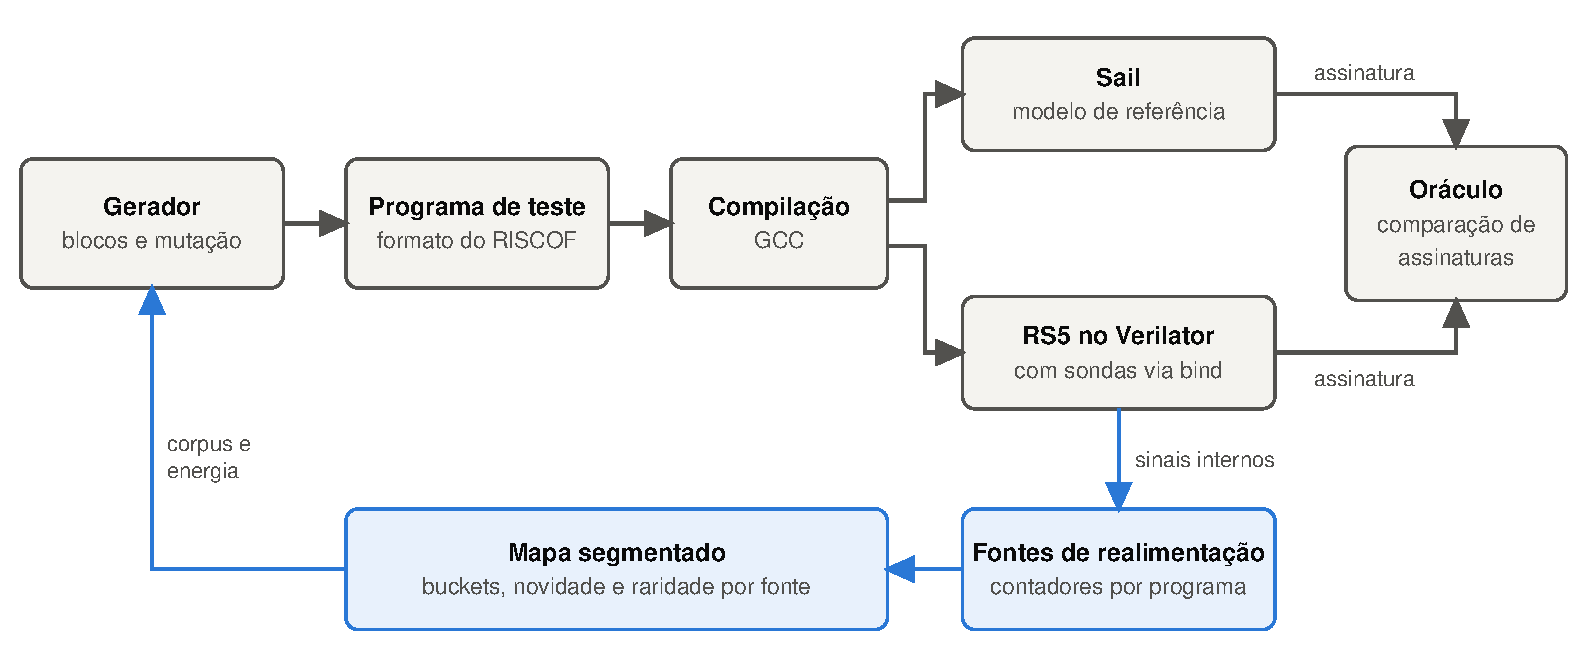
\includegraphics[width=\textwidth]{fig/fluxo_fuzzer.pdf}
    \caption{Fluxo de um programa no \textit{fuzzer}. Em azul, o laço de realimentação.}
    \label{fig:fluxo}
\end{figure}

Um programa é composto por um prólogo, que inicializa os registradores e uma região de memória, por três a oito blocos e por um epílogo, que grava os registradores na assinatura. Nesta versão preliminar os blocos são sintéticos e organizados por classe de instrução: operações lógicas e aritméticas, acessos à memória, multiplicação e divisão, desvios, laços, saltos e acessos a CSRs. Cada bloco favorece o uso de registradores escritos há pouco, para formar dependências entre instruções. O corpus de blocos extraídos de aplicações reais, previsto nos objetivos, substituirá esses blocos. As mutações atuam sobre blocos inteiros: substituição, inserção, remoção, troca de posição, recombinação entre dois programas e alteração dos valores iniciais. Quando há corpus, 80\% dos programas são mutações de um pai sorteado conforme sua energia, e os demais são gerados do zero.

Uma segunda versão do gerador acrescenta \textit{traps}. O programa passa a incluir um tratador que registra a causa na assinatura, avança sobre a instrução que a provocou e retorna. O gerador ganha três tipos de bloco: exceções (chamadas de sistema, instruções ilegais, escritas em CSRs somente de leitura e acessos desalinhados), interrupções de temporizador habilitadas em torno de uma a três instruções, e trechos executados em modo de usuário. Valores que diferem legitimamente entre o RS5 e o Sail não chegam à assinatura, como os contadores de desempenho e o endereço de retorno de uma interrupção, que depende do ciclo em que ela é aceita.

As fontes são capturadas por módulos SystemVerilog ligados ao RS5 pela construção \texttt{bind}, sem alteração do RTL. Cada fonte ocupa uma região do mapa, com contadores gravados ao final da simulação, e o \textit{fuzzer} aplica a cada região a regra de \textit{buckets} e de novidade. Todas as fontes são registradas em todas as execuções; a linha de comando define quais delas decidem a entrada no corpus e a energia, e a geração sem realimentação é o mesmo \textit{fuzzer} com esse conjunto vazio. As sondas custam cerca de 1~ms por programa, 5\% do tempo de simulação, enquanto a instrumentação de cobertura do Verilator triplica esse tempo, de 18,5 para 54,9~ms.

\section{Experimentos}\label{sec:previo-exp}

Os experimentos usaram o RS5 na configuração RV32IM com Zicsr e Zihpm, modos de máquina e de usuário, predição de desvios e encaminhamento habilitados, fila de duas instruções e memória de dados com dois ciclos de latência, escolhida por ativar o \textit{stall}. Foram executados cerca de 1,8 milhão de programas em três campanhas: duas com rodadas de 8.000 programas, para comparar as fontes e os geradores, e uma com rodadas de 200.000 programas, para observar a saturação. Os grupos principais foram repetidos com três sementes. Entre as rodadas de uma comparação, o gerador e a semente são mantidos, e apenas a fonte que guia a exploração muda. O objetivo desses experimentos é comparar as fontes, e não avaliar o \textit{fuzzer} final: o gerador e as mutações utilizados são provisórios.

\subsection{Saturação das fontes}\label{sec:previo-sat}

A \cref{tab:saturacao} resume o comportamento de cada fonte sob geração aleatória com o gerador com \textit{traps}. As posições são os elementos distintos que a fonte registrou: pontos de cobertura, \textit{bins}, transições ou arestas.

\begin{table}[H]
    \centering
    \caption{Saturação das fontes em 200.000 programas aleatórios (três sementes). As colunas de 50\% e 90\% indicam quantos programas foram necessários para atingir essa fração do total observado.}
    \label{tab:saturacao}
    \small
    \begin{tabular}{|l|r|r|r|r|}
        \hline
        \textbf{Fonte} & \textbf{Posições} & \textbf{50\%} & \textbf{90\%} & \textbf{Novas nos últimos 10.000} \\
        \hline
        Cobertura do Verilator$^{*}$ & 1.052 & 2 a 4 & 61 a 64 & 0 \\
        \hline
        \textit{Bins} & 49 de 64 & 2 a 3 & 34 a 73 & 0 \\
        \hline
        Transições de CSRs & 978 $\pm$ 3 & 2.100 a 2.600 & 56.000 a 57.000 & 2 a 6 \\
        \hline
        Arestas do \textit{pipeline} & 30.736 $\pm$ 40 & 9.400 a 9.600 & 107.000 a 108.000 & 238 a 253 \\
        \hline
        \multicolumn{5}{l}{\footnotesize $^{*}$ Medida em rodadas de 8.000 programas, por causa do custo da instrumentação.}
    \end{tabular}
\end{table}

A cobertura do Verilator e os \textit{bins} esgotam-se em centenas de programas. A partir desse ponto todo programa repete o que já foi visto, e a fonte deixa de distinguir um programa de outro. Os 15 \textit{bins} restantes permaneceram em zero nos 600.000 programas das três sementes. As transições de CSRs formam um espaço de cerca de mil posições, quase todo observado ao fim das rodadas. As arestas do \textit{pipeline} são a única fonte que continua a crescer: ao fim de 200.000 programas ainda surgem cerca de 250 arestas novas a cada 10.000. O estimador Chao1 \citep{chao1984}, aplicado ao número de arestas vistas em um e em dois programas, indica cerca de 35 mil arestas alcançáveis por esse gerador, das quais 87\% foram observadas. As três sementes diferem em menos de 0,3\% no total, o que mostra que esses números são propriedade do gerador, e não do acaso.

\subsection{Geração aleatória e geração guiada}\label{sec:previo-guiada}

A \cref{fig:saturacao} compara quatro formas de gerar 200.000 programas. Nas duas primeiras não há realimentação, e o que muda é o gerador, sem e com \textit{traps}. Na terceira, as arestas do \textit{pipeline} guiam a exploração. A quarta isola o efeito do sinal: aplica as mesmas mutações, na mesma proporção, mas admite todo programa no corpus e sorteia os pais ao acaso.

\begin{figure}[htb]
    \centering
    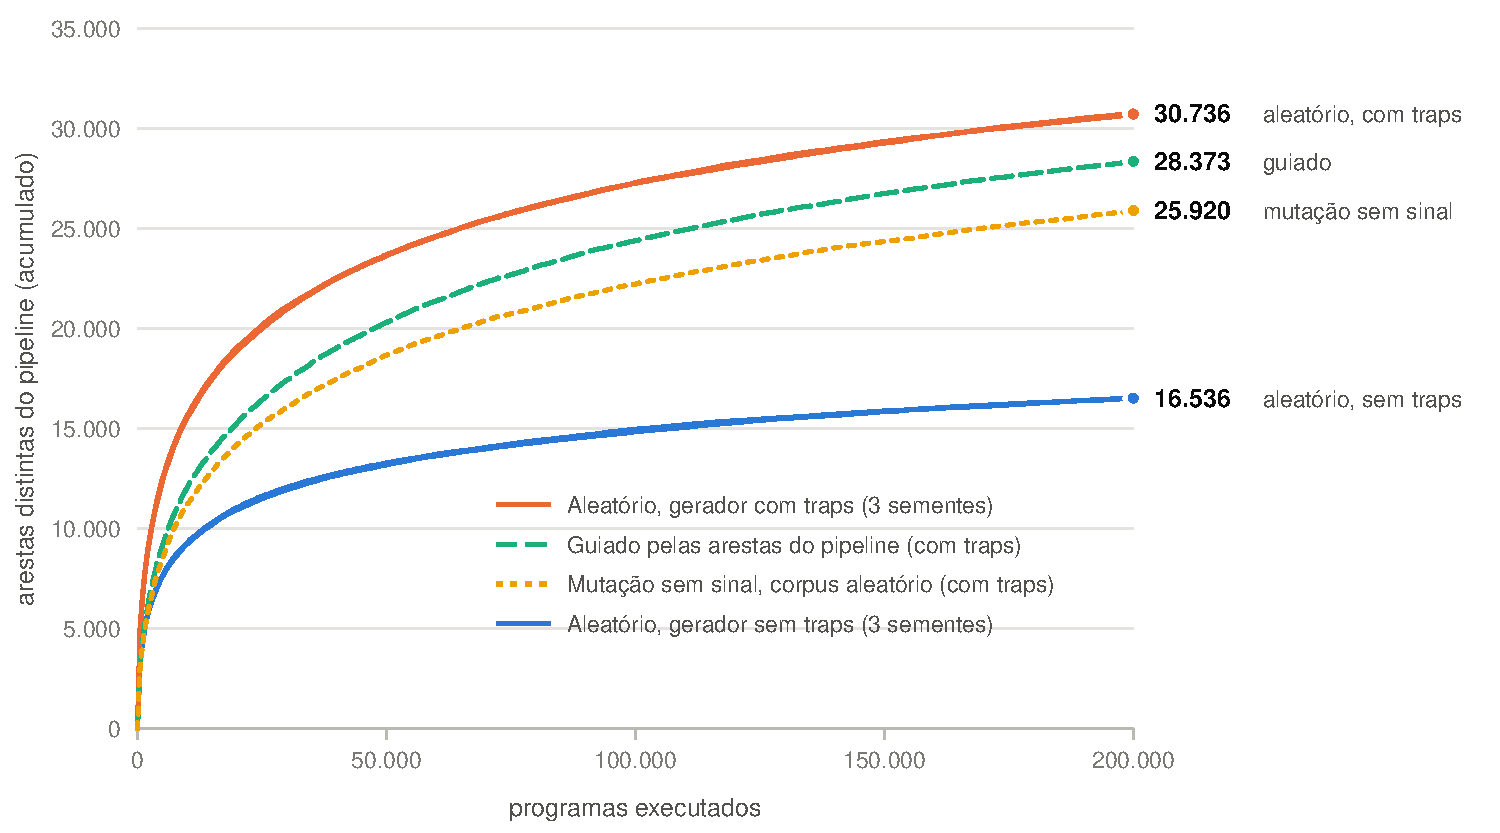
\includegraphics[width=\textwidth]{fig/saturacao_arestas.pdf}
    \caption{Arestas distintas do \textit{pipeline} acumuladas ao longo de 200.000 programas. As rodadas aleatórias têm três sementes cada, que se sobrepõem.}
    \label{fig:saturacao}
\end{figure}

Com 8.000 programas, a rodada guiada alcançou 76\% das arestas da aleatória (11.085 contra 14.573). A causa é a mutação, e não o sinal. Um programa gerado do zero trouxe em média 3,8 arestas novas, contra 0,2 a 1,2 de um programa mutado, e a perda cresceu na proporção dos programas mutados quando essa fração foi variada. Com o mesmo mutador, escolher os pais pelo sinal rendeu mais arestas do que escolhê-los ao acaso nas três sementes testadas.

A diferença para a geração aleatória diminui continuamente com o orçamento, como mostra a \cref{fig:razao}: a rodada guiada tem 66\% das arestas da aleatória com 1.000 programas, 76\% com 8.000, 86\% com 50.000 e 92\% com 200.000. Nos últimos 50.000 programas ela acrescentou 1.607 arestas, contra 1.388 a 1.427 das rodadas aleatórias. A vantagem do sinal sobre a mutação sem sinal também cresce, de 7\% para 9,5\%.

\begin{figure}[htb]
    \centering
    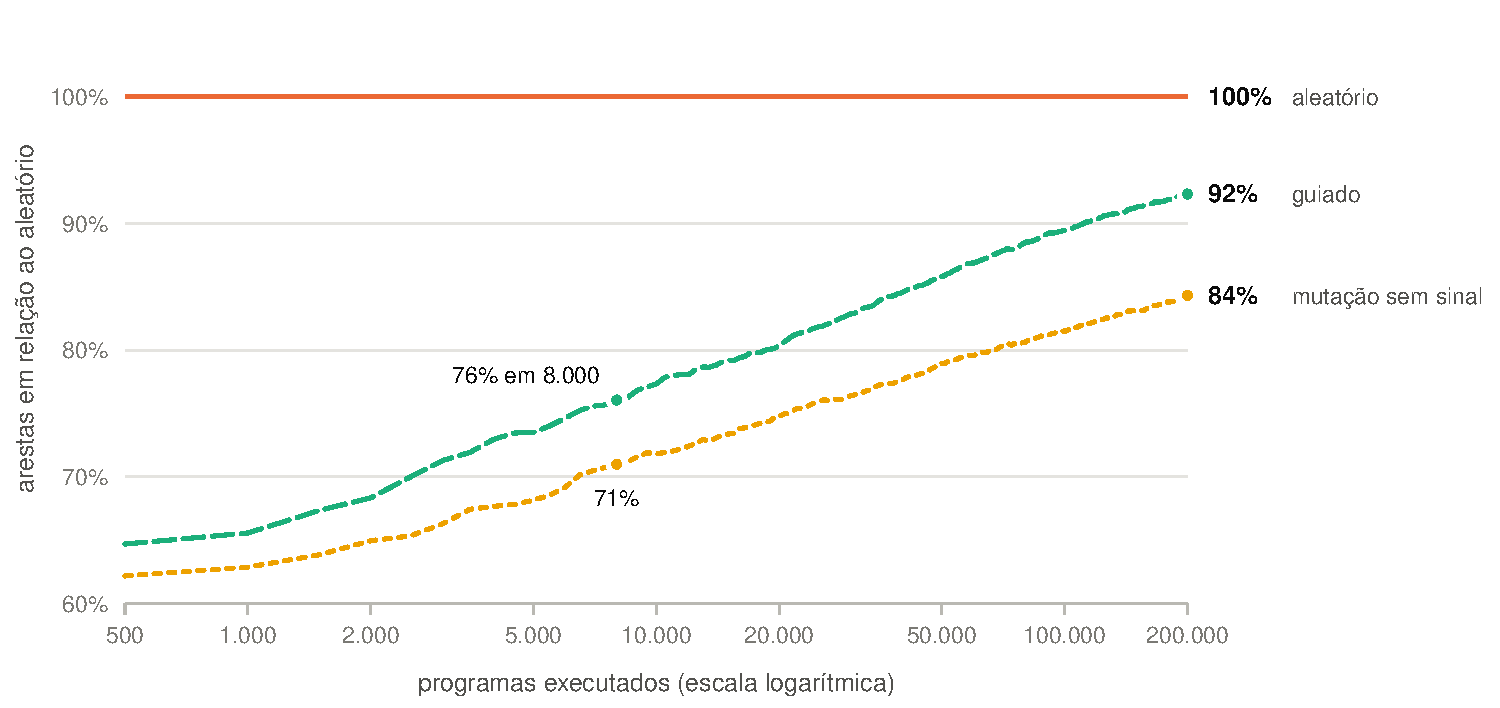
\includegraphics[width=\textwidth]{fig/razao_guiado.pdf}
    \caption{Arestas alcançadas com mutação, em relação à média das três rodadas aleatórias com o mesmo gerador.}
    \label{fig:razao}
\end{figure}

A realimentação muda sobretudo o tratamento dos estados raros. Na rodada aleatória, 16\% das arestas foram vistas em um único programa; na guiada, 5,6\%. Das 11.815 arestas que apareceram em no máximo cinco dos 200.000 programas de uma rodada aleatória, a rodada guiada alcançou 7.052 e exercitou cada uma em seis programas, na mediana, enquanto outra rodada aleatória alcançou 8.533, em dois programas cada. Em relação a 400.000 programas aleatórios, uma nova rodada aleatória contribui com 1.745 a 1.806 arestas inéditas, a rodada guiada com 1.603 a 1.729 e a mutação sem sinal com 629 a 850. Com 8.000 programas, a contribuição da rodada guiada era cerca de metade da de uma rodada aleatória (966 a 1.170 contra 2.007 a 2.067) e pouco superior à da mutação sem sinal. Portanto, dentro do orçamento medido, a rodada guiada não superou a aleatória no total de estados, e não há evidência de que ela alcance estados inacessíveis à geração aleatória. O que os dados mostram é que sua desvantagem inicial se reduz de forma contínua e que ela revisita os estados raros com mais frequência.

Duas características da infraestrutura preliminar explicam a vantagem da geração aleatória. A primeira é o mutador: como cada mutação preserva a maior parte do programa de origem, um programa mutado repete quase todos os estados do pai. A segunda é o espaço de estados produzido pelo gerador, que é raso. As arestas raras são, em sua maioria, combinações de características independentes, como a origem do encaminhamento, o nível da fila e a classe da instrução, e não situações que dependam de uma sequência anterior específica. Em um espaço assim, sortear programas novos cobre bem as combinações, e há pouco a ganhar em partir de um programa que já chegou a um estado raro.

Uma limitação dessas medidas é o tamanho do mapa: com $2^{16}$ posições, de 5\% a 8\% das posições das arestas sofreram colisão, o que subestima os totais de todas as rodadas. O mapa será ampliado nas próximas campanhas.

\subsection{Divergência encontrada}\label{sec:previo-bug}

Nenhum dos 80.000 programas sem \textit{traps} da segunda campanha divergiu do Sail. Com \textit{traps}, 354 de 80.000 divergiram, todos pela mesma causa. Quando um programa habilita a interrupção de temporizador, executa uma instrução e desabilita as interrupções com uma escrita em \texttt{mstatus}, o RS5 aceita a interrupção no ciclo em que essa escrita termina. A atualização de \texttt{mstatus} pela entrada no \textit{trap} tem prioridade sobre a escrita da instrução, que se perde: após o retorno, as interrupções estão habilitadas no RS5 e desabilitadas no Sail. A divergência foi reproduzida por um teste dirigido com oito variantes da sequência e não depende da latência da memória. Nas rodadas de 200.000 programas, ela foi disparada por 0,37\% a 0,40\% dos programas aleatórios.

A \cref{tab:bug} mostra quantos programas dispararam a divergência conforme a fonte que guiou a rodada.

\begin{table}[H]
    \centering
    \caption{Programas que dispararam a divergência em rodadas de 8.000 programas com o gerador com \textit{traps}.}
    \label{tab:bug}
    \small
    \begin{tabular}{|l|r|r|}
        \hline
        \textbf{Realimentação} & \textbf{Programas que dispararam} & \textbf{Programa do décimo disparo} \\
        \hline
        Nenhuma (três sementes) & 25, 30 e 33 & 2.424 a 3.388 \\
        \hline
        Arestas do \textit{pipeline} & 27 & 2.982 \\
        \hline
        Transições de CSRs & 131 & 756 \\
        \hline
        Mutação sem sinal & 14 & 5.517 \\
        \hline
    \end{tabular}
\end{table}

A rodada guiada pelas transições de CSRs disparou a divergência quatro vezes mais do que as aleatórias e chegou ao décimo disparo bem antes delas. A rodada guiada pelas arestas do \textit{pipeline} não se distinguiu da geração aleatória. Trata-se de uma única falha, mas o resultado indica que a fonte que acumula mais estados não é necessariamente a que mais dispara uma falha: a métrica de CSRs distingue exatamente os estados em que essa falha se manifesta.

\section{Considerações}\label{sec:previo-remarks}

O resultado mais nítido é o peso do gerador. Acrescentar \textit{traps} ampliou as arestas observadas em 86\% (de 16.536 para 30.736), as transições de CSRs de 584 para 978 e os \textit{bins} atingidos de 31 para 49, e somente os programas com \textit{traps} revelaram a divergência. Nenhuma fonte de realimentação produziu efeito comparável, e nenhuma quantidade de programas alcançou os \textit{bins} que o gerador não sabe produzir. Isso está de acordo com o Encarsia, segundo o qual os programas gerados determinam quais falhas são encontradas, mais do que o mecanismo de realimentação.

Os \textit{traps} importam também pelo que exercitam. Exceções, interrupções e retornos são o caminho pelo qual o processador muda de modo de privilégio, e a separação entre os modos de máquina e de usuário depende de que esse estado seja atualizado corretamente. A divergência encontrada pertence a essa classe: um programa que desabilita as interrupções para proteger uma região crítica prossegue com elas habilitadas. Como observa o Encarsia, toda falha arquiteturalmente observável pode ter implicações de segurança, e as falhas no estado privilegiado são as de consequência mais direta.

Quanto às fontes, as arestas do \textit{pipeline} serão a fonte principal do \textit{fuzzer}: é a única que não se esgota, mantém resolução para distinguir programas ao longo de toda a campanha e corresponde à realimentação funcional que o Encarsia recomenda. As transições de CSRs serão usadas como fonte complementar. Seu espaço é pequeno, mas ela favoreceu a única falha encontrada, o que é coerente com a proposta do ProcessorFuzz nesse caso e não contradiz o Encarsia, cujo resultado se refere a conjuntos de falhas distribuídas pelo projeto. A cobertura do Verilator fica restrita ao relato dos resultados, e os \textit{bins}, ao diagnóstico do gerador.

Os experimentos deste capítulo não avaliam o \textit{fuzzer} proposto: são um estudo da saturação das fontes, feito com um gerador e um mutador provisórios. Nesse cenário a exploração guiada ficou abaixo da geração aleatória no total de estados, pelas duas limitações apontadas na \cref{sec:previo-guiada}. Ambas pertencem ao gerador, e não ao sinal, e a tendência medida é favorável: a desvantagem cai de 34\% para 8\% entre 1.000 e 200.000 programas, e a escolha dos pais pelo sinal supera a escolha ao acaso em todos os orçamentos. Por isso, a proposta para a continuidade do trabalho é melhorar o gerador e a mutação até que a exploração guiada supere a geração aleatória nos estados alcançados. Espera-se que o corpus de blocos extraídos de aplicações reais aprofunde o espaço de estados, por trazer cadeias de dependência mais longas entre as instruções, e os operadores de mutação passarão a alterar mais de um bloco, para que um programa mutado se afaste mais de sua origem. A hipótese é que, em um espaço mais profundo, partir dos programas que alcançaram estados raros renda mais do que sortear programas novos.

O número de estados, porém, é uma medida intermediária: o que se quer do \textit{fuzzer} são falhas encontradas, e até aqui há uma única divergência para sustentar qualquer conclusão nesse sentido. A resposta também depende do orçamento, pois com 8.000 programas a realimentação parece prejudicial e só em campanhas longas sua desvantagem se reduz. O \textit{fuzzer} final será avaliado pelo tempo até a detecção de falhas injetadas no RS5, uma por vez, como propõe o Encarsia, com curvas ao longo do orçamento em lugar de um único ponto e com a geração aleatória como linha de base em todas as comparações.


% ---------------------------------------------------------------------------
% Roteiro original do capítulo (mantido como referência)
% ---------------------------------------------------------------------------
% \chapter{Trabalho previo - sugerir titulo para o capitulo}
% 
% - Levantamento de sinais para servir como feedback do fuzzer
%     * Random -> usado como baseline
%     * Coverage do SystemVerilog
%     * Estado do pipeline -> OK, apontar para seção que vai detalhar os experimentos
%         -> Como é um core pequeno, diferencial que pode mapear o pipeline
%     * CSRs (valores contidos neles)
%         -> Relacionar ProcessorFuzz com Encarsia - um é oposto do outro, ref com a seção de experimentos
%     * Bins (propriedades relacionadas entre sinais/registradores) -> justificar por que não foi usado
%         -> Dá hints da microarquitetura - não é o que procuramos aqui
%         -> Da muito vies do programador (tentar achar uma referencia aqui)
% 
% - Descrever como foi implementado o fuzzer e como ele funciona em conjunto com o RISCOF
% 
% - Descrição dos experimentos e resultados
%     * Random vs. guided - experimentos
%     * Gráficos
%     * Resultados
%     * Falar que com 8000 testes o guided perdeu para o random em estados totais, mas com mais testes ele ganha (o guided consegue achar estados raros, enquanto o random nao, por isso ele ultrapassa)
% 
% - Seção final de 'remarks'
%     * Gerador com traps -- Encarsia cita que o gerador é mais importante (tao importante quanto) o feedback - segue o que foi encontrado
%         -> É importante a parte de traps devido ao teste de privilégios (modos) de execução - bug é falha de segurança!!!!!
